\documentclass[12pt]{article}
% \documentclass[12pt, twocolumn]{article}
\usepackage[margin=2.5cm]{geometry}
\usepackage{enumerate, fancyhdr, graphicx, amsmath, lipsum, wrapfig, nameref, url, hyperref,
            setspace, color, csquotes, textcomp, subcaption, float }

\title{Mars Landing Site Traversability}
\author{Paul Chesnais (pmc85)}
\date{\today}

\pagestyle{fancy}
\fancyhead{}
\lhead{Paul Chesnais (pmc85)}
\chead{Mars Landing Site Traversability}
\rhead{\today}
\fancyfoot{}
\rfoot{\thepage}
\lfoot{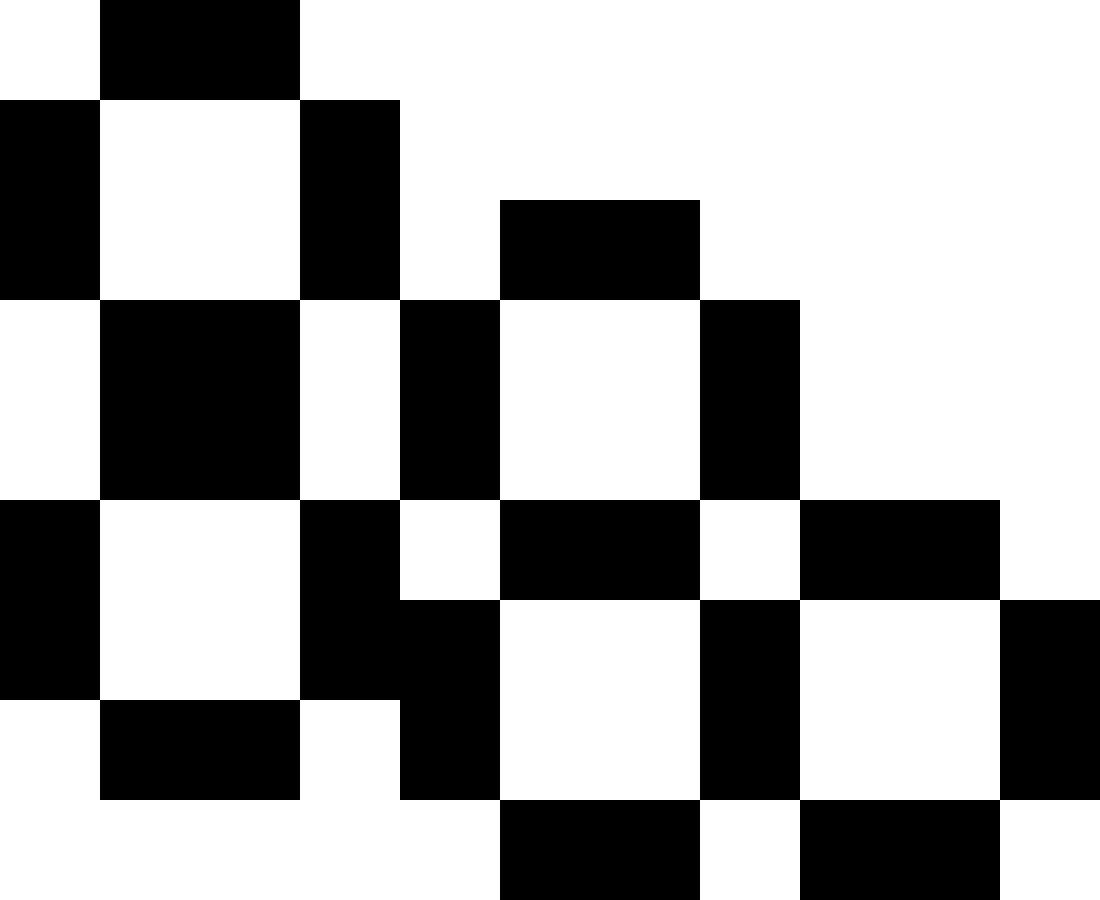
\includegraphics[height=20pt]{Logo}}
\renewcommand{\headrulewidth}{0.5pt}
\renewcommand{\footrulewidth}{0.5pt}
% \onehalfspacing

\usepackage[binary-units=true]{siunitx}
\sisetup{load-configurations = abbreviations}

\newcommand{\p}[1]{\times 10^{#1}}
\newcommand{\supcite}[1]{\textsuperscript{\cite{#1}}}
\newcommand{\MATLAB}{MATLAB\textsuperscript{\textregistered}}

\begin{document}
\maketitle
\thispagestyle{empty}

\section{Abstract}
\label{sec:abstract}
Exploring a planet on the ground isn't easy. Especially since as of right now, rovers are the only things capable of doing it. Unfortunately, designing rovers is incredibly difficult. Given the topology for a particular landing site, how do you optimize each component of a rover? Some of these components govern how steep a slope the rover can climb or make its way down on. This project aims to illustrate how ``agile'' Mars rovers should be by computing traversability maps of candidate landing sites.

\section{Datasets}
\label{sec:datasets}
\par For the purposes of this project, we need a dataset that is accurate on a scale that is reasonable relative to the Rover's size. Curiosity was 3 meters long\supcite{bib:curiosity}, and the Mars 2020 rover is also expected to be 3 meters long\supcite{bib:rover2020}. This dictates the order of the resolution of the datasets required for this study to be meaningful. Suppose we had a topographical map with a horizontal resolution on the scale of 20 meters or even 10 meters between data points. Unfortunately, insurmountable rocks and obstacles do come in all shapes and sizes, many of which smaller than 20 meters. Such a map would not necessarily reflect the presence of these obstacles and pose an unforeseen problem to rover. This effectively leaves us with two choices in topographical maps: HSRC DTMs (Digital Topographical Maps) from the Mars Express mission, or HiRISE DTMs from the Mars Reconnaissance Orbiter mission. HSRC DTMs are on the scale of 2 meters per pixel\supcite{bib:hsrc} and HiRISE DTMs are on the accuracy of 1 meter per pixel\supcite{bib:abouthirise}. For the sake of this study's rigor, the decision was made to use the more recent and more accurate HiRISE DTMs. Given that the horizontal resolution of those DTMs is three times smaller than the length of the rover and that their vertical accuracy is ``in the tens of centimeters''\supcite{bib:abouthirise}, any unforeseen obstacles should be small, flat, and, in theory, relatively easy to avoid.
\par Figure~\ref{fig:dtms} is a table showing which datasets were used, their respective identifiers, resolutions and area of coverage. It is noted that not all candidate landing sites were covered and presented in this proposal, but the algorithm is robust and is designed to be used with all HiRISE DTMs. The datasets were selected for their interesting features and potentially treacherous terrain. Please visit the code's \href{https://github.com/PapaCharlie/Rover-Climb-Angles/tree/master/figures/maps/}{\ttfamily\color{blue} \underline{source}} for more maps.
\par The number of pixels is quoted to highlight the complexity of the data we will be working with. Additionally, each pixel is stored as 64-bit floating point number in memory. In other words, each dataset occupies more than 1 GB of ram, making them tricky to work with in most languages. The value of each pixel represents its vertical distance from a theoretical, well defined sphere surrounding Mars. Not every DTM uses a sphere of the same radius, but each DTM is consistent throughout. Therefore subtracting the value of one pixel from its neighbor gives us the difference in height between the two.
\par The average coverage is $\SI{103.15}{\kilo\meter\squared}$, which may seem small, but given that Curiosity's ground speed is about $\SI{0.14}{\kilo\meter\per\hour}$, it would take close to 500 days nonstop to visit every single point.
\begin{figure*}
  \center
  \begin{tabular}[b]{c|c|c|c|c}
    Name & Dataset & Pixels & Resolution & Area covered \\ \hline
    Southwest Arabia Terra &  ESP\_011844\_1855\supcite{bib:ESP_011844_1855} & 1.74e+08 & 1.011655 & $\SI{107.39}{\kilo\meter\squared}$\\
    Gale Crater &             ESP\_023957\_1755\supcite{bib:ESP_023957_1755} & 1.14e+08 & 1.011763 & $\SI{79.47}{\kilo\meter\squared}$\\
    Holden Crater &           ESP\_019612\_1535\supcite{bib:ESP_019612_1535} & 1.90e+08 & 1.007219 & $\SI{122.50}{\kilo\meter\squared}$\\
    Eberswalde Crater &       ESP\_019757\_1560\supcite{bib:ESP_019757_1560} & 1.64e+08 & 1.008208 & $\SI{110.22}{\kilo\meter\squared}$\\
    Mawrth Vallis &           ESP\_015985\_2040\supcite{bib:ESP_015985_2040} & 1.33e+08 & 1.008208 & $\SI{96.15}{\kilo\meter\squared}$\\
  \end{tabular}
  \caption{DTMs used and their respective properties}
  \label{fig:dtms}
\end{figure*}

\section{Method}
\label{sec:method}
\subsection{Modified Dijkstra's Algorithm}
\label{sub:the_algorithm}
\par The algorithm used was inspired by the single-source version of Dijkstra's algorithm. Dijkstra's algorithm is an algorithm used to find the shortest path from the starting node to a given node. The single-source version
is a generalization that finds the shortest path from a given starting node to all the nodes in a graph. This modified version of the algorithm finds the flattest path between two points, i.e. the path that requires the flattest climbing angle. The ``required'' angle, in this case, would be the angle of the steepest slope along the path between the two points.
\par Suppose we have a graph representing a topographical map, with $V$ the set of all nodes in the graph, and $E$ the set of all edges. Each node in the graph represents a physical location and its associated altitude. For notation, let the height of a given node $u$ be returned by $height(u)$, the function $d(u.v)$ be the function that returns the physical distance between $u$ and $v$, and the function $angle(u,v)$ be the function that returns the angle of the slope between points $u$ and $v$. For any two connected nodes $u$ and $v$, the value of the edge $(u,v)$ that connects them is $angle(u,v)$. Finally, for two nodes $u$ and $v$, we have:
\begin{align*}
  angle(u,v) = \tan^{-1}\left(\frac{height(u) - height(v)}{d(u,v)}\right)
\end{align*}
\pagebreak
\par We also define a data structure, called a Frontier, that contains pairs of nodes and angles. Let us define a series of functions for this data structure, where $fr$ is a Frontier:
\begin{itemize}
  \item For a node $v$ and an angle $\alpha$, let $push(fr, (v,\alpha))$ add the pair $(v, \alpha)$ to the Frontier $fr$. If there exists a pair $(v,\beta)$ in $fr$ such that $|\alpha| \leq |\beta|$, remove the pair $(v,\beta)$ and add the pair $(v,\alpha$.
  \item Let $pop(fr)$ return the pair $(v, \alpha)$ such that for pairs $(u,\beta)$ in $fr$: $|\alpha| \leq |\beta|$.
  \item Let $\|fr\|$ be the number of pairs contained in $fr$.
\end{itemize}
\par We can use the above to express the modified Dijkstra's algorithm, given an arbitrary starting node $s$:
\begin{enumerate}[Step 1]
  \item Define an array $required$ such that $required[v]$ returns the flattest required angle for the paths that connect $s$ to $v$. Because no nodes have been visited yet, set $required[v] = +\infty$ for all nodes $v$ in the set $V$. Define an empty Frontier $fr$.
  \item Visit $s$, i.e. execute $push(fr, (s, 0))$ and set $required[s] := 0$.
  \item Let $(v,\alpha) = pop(fr)$. For all each neighbor $n$ of $v$, do the following:
  \begin{displayquote}
    Let $\alpha := angle(v,n)$ if $|required[v]| < |angle(v,n)|)$, otherwise $\alpha := required[v]$. If $ |\alpha| < |required[n]|$: set $required[n] := \alpha$ and $push(fr, (n, \alpha))$.
  \end{displayquote}
  Repeat Step 3 until $|fr| == 0$
\end{enumerate}
\par For this algorithm, the Frontier represents the the set of nodes that we can reach from the set of nodes that we've explored. By popping the flattest pair from the Frontier every time, we guarantee that the associated required angle for each node on the frontier is the flattest possible. Suppose two neighboring nodes $u$ and $v$, such that $required[v] = 0$, $|angle(v,u) > 0|$, and $u$ has not yet been visited. The value set at $required[u]$ must be $angle(v,u)$, otherwise $u$ will inherit a flatter angle than what is required in reality. Therefore Step 3 maintains the correctness of the traversal by setting the value in $required$ to be whichever angle is steeper between $required[v]$ and $angle(v,n)$. With the guarantees maintained by Step 3 and the Frontier data structure, every time we associate a required angle to a given node, said angle is the flattest, and the final $required$ contains the correct values for all nodes.

\subsection{Using the data}
\label{sub:using_the_data}
\par First, we want to represent the Graph explained above using the data. In this case, each pixel is a node $p$ and $height(p)$ is simply the value in the DTM at the position $p$. Next, each pixel is connected to its 4 closest neighbors, i.e. the pixels that are directly in contact with it. To avoid interpolation and potential errors, pixels are not connected to diagonal neighbors. As such, we can also set $d(u,v)$ to always be equal to the horizontal resolution in the dataset for any two neighboring pixels $u$ and $v$. The starting position $s$ will be naively chosen to be the pixel at the center of the DTM.
\par Next, we need to provide an implementation of the Frontier data structure, to the same specifications as defined above. In this case, a MinHeap is ideal because it fits the exact criteria. A MinHeap is a balanced data structure, where $push$ and $pop$ operations require that the MinHeap be rebalanced. If there are $n$ elements in the MinHeap, then rebalancing the MinHeap will take at worst $\log_2(n)$ operations. This means that finding the flattest pair in the MinHeap can be done very quickly with little overhead. Since our DTMs usually have more than 100 million pixels and the frontier of visited pixels can grow arbitrarily large, fast $push$ and $pop$ operations become crucial.
\par Finally, we need to create the $required$ array. This is easily done by creating an array the same size as the DTM, then indexing into it exactly like we index into the DTM. Unfortunately, these operations become computationally expensive quite quickly. If the DTM takes 1 GB in memory, so will the $required$ array. Additionally, as said before, the Frontier can grow arbitrarily large. As such, in the absolute worst case scenario, computing the traversability map can require up to 3 GB of memory at runtime. This causes a lot of issues because not all of the data can be loaded into the processor's more restricted memory at a time, meaning that a lot of time is spent waiting for data from RAM. Fortunately, Modern RAM responds quite quickly and data usually will take a handful of CPU cycles to arrive.

\subsection{Optimizations}
\label{sub:optimizations}
\par There was an initial, fruitless attempt at implementing this in \MATLAB{}. To illustrate the speed of the process, the program gave periodic progress updates in the form of messages saying that a certain integer percent of the pixels had been visited. Unfortunately, these progress updates came at the rate of about once every hour, leading one to believe that iterating over all of the datasets could, and most likely would, take weeks. Clearly, a radical change need to be made.
\par As such, \MATLAB{} was dropped, and Golang became the language of choice. Because Golang is compiled, the same program was expected to run more efficiently. The current implementation of the algorithm takes less than 2 minutes to compute the entire traversability map. An immense, unexpected, yet welcome change in runtime meant that we could move on at a more reasonable pace.
% Other, smaller, optimizations were made. For example, computing trigonometric functions is computationally expensive because it requires approximating an infinite sum. As such, instead of computing the arc tangent of the difference in height between two neighbors over the resolution, only the difference in height was recorded.

\subsection{Data Pipeline}
\label{sub:data_pipeline}
\par HiRISE DTMs come in the form of IMG files. This meant that they needed to be converted into a format that was readable by Golang. Golang already has a library that can read FITS files. As such, the USGS ISIS software package was used to convert the IMG files into FITS files. Then it is a simple matter of extracting the resolution and image size from the label included in the IMG file to get all the information required to compute the map.
\par Once the algorithm has run its course, it saves the map to disk in a format that is readable by \MATLAB{}. The map is loaded into memory and stretched between -20\textdegree and 20\textdegree to show detail, under the assumption that rovers cannot, or prefer not to, climb slopes past those angles. Finally, what we will call a traversability histogram is plotted. A traversability histogram is a histogram that shows required angle versus number of pixels. To find the area a given rover can cover, integrate the histogram between the bounds $\alpha$ and $\beta$ where $\alpha$ and $\beta$ are respectively the steepest negative and positive angles the rover can climb. The shaded area represents the range of required angles to access 95\% of the landing site.

\section{Results}
\label{sec:results}
\par We can finally begin presenting the results of our hard work.
\subsection{Southwest Arabia Terra\supcite{bib:ESP_011844_1855}}
\label{sub:southwest_arabia_terra}
\begin{figure}[h!]
  \centering
  \begin{subfigure}[t]{0.27\textwidth}
    \centering
    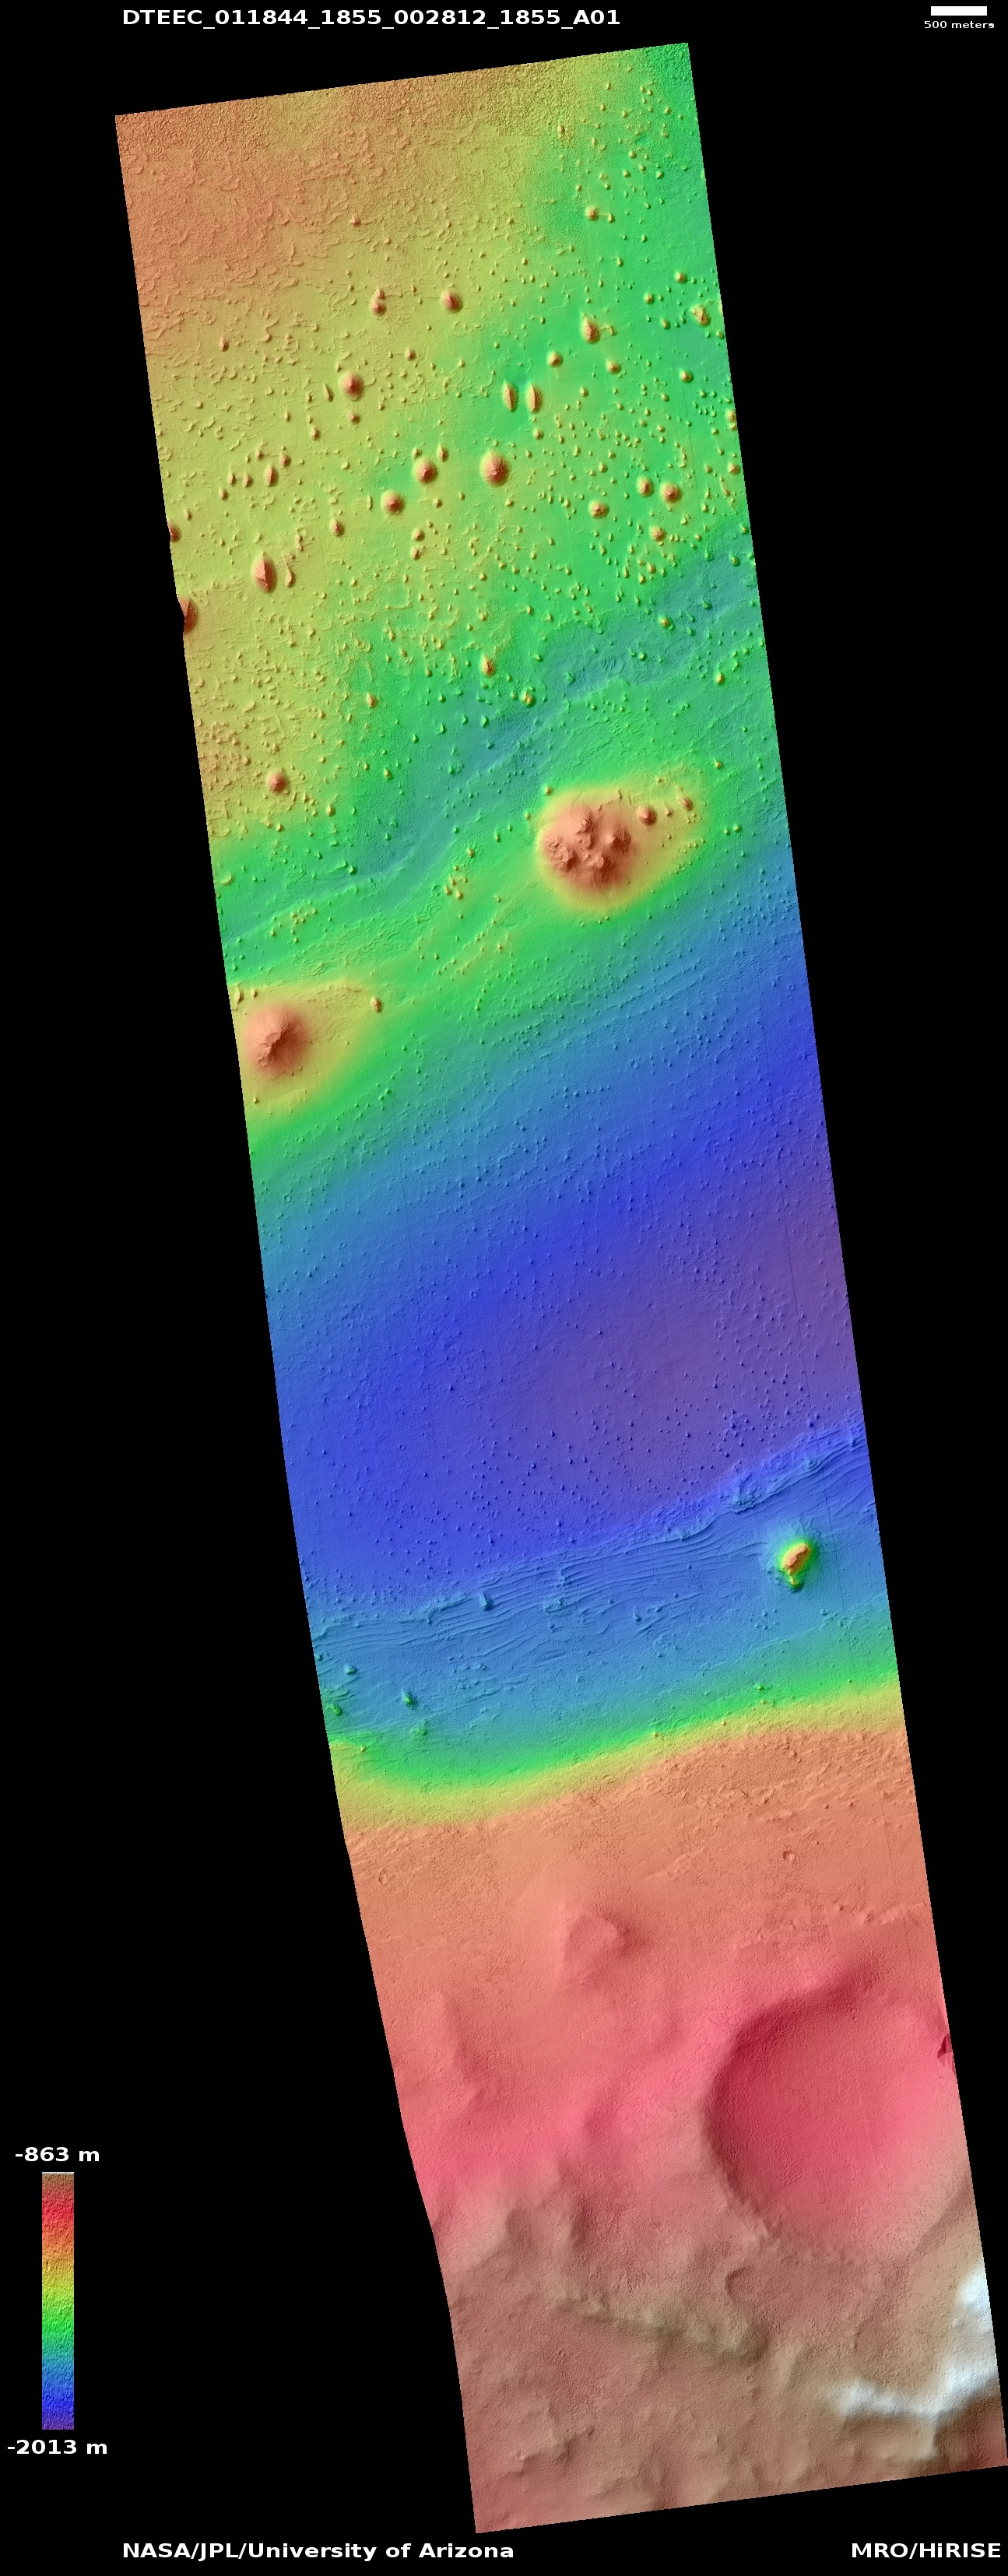
\includegraphics[height=0.4\paperheight]{figures/maps/ESP_011844_1855/DTEEC_011844_1855_002812_1855_A01.jpg}
    \caption{Color altimetry map}
    \label{fig:southwest_dtm}
  \end{subfigure}
  ~
  \begin{subfigure}[t]{0.27\textwidth}
    \centering
    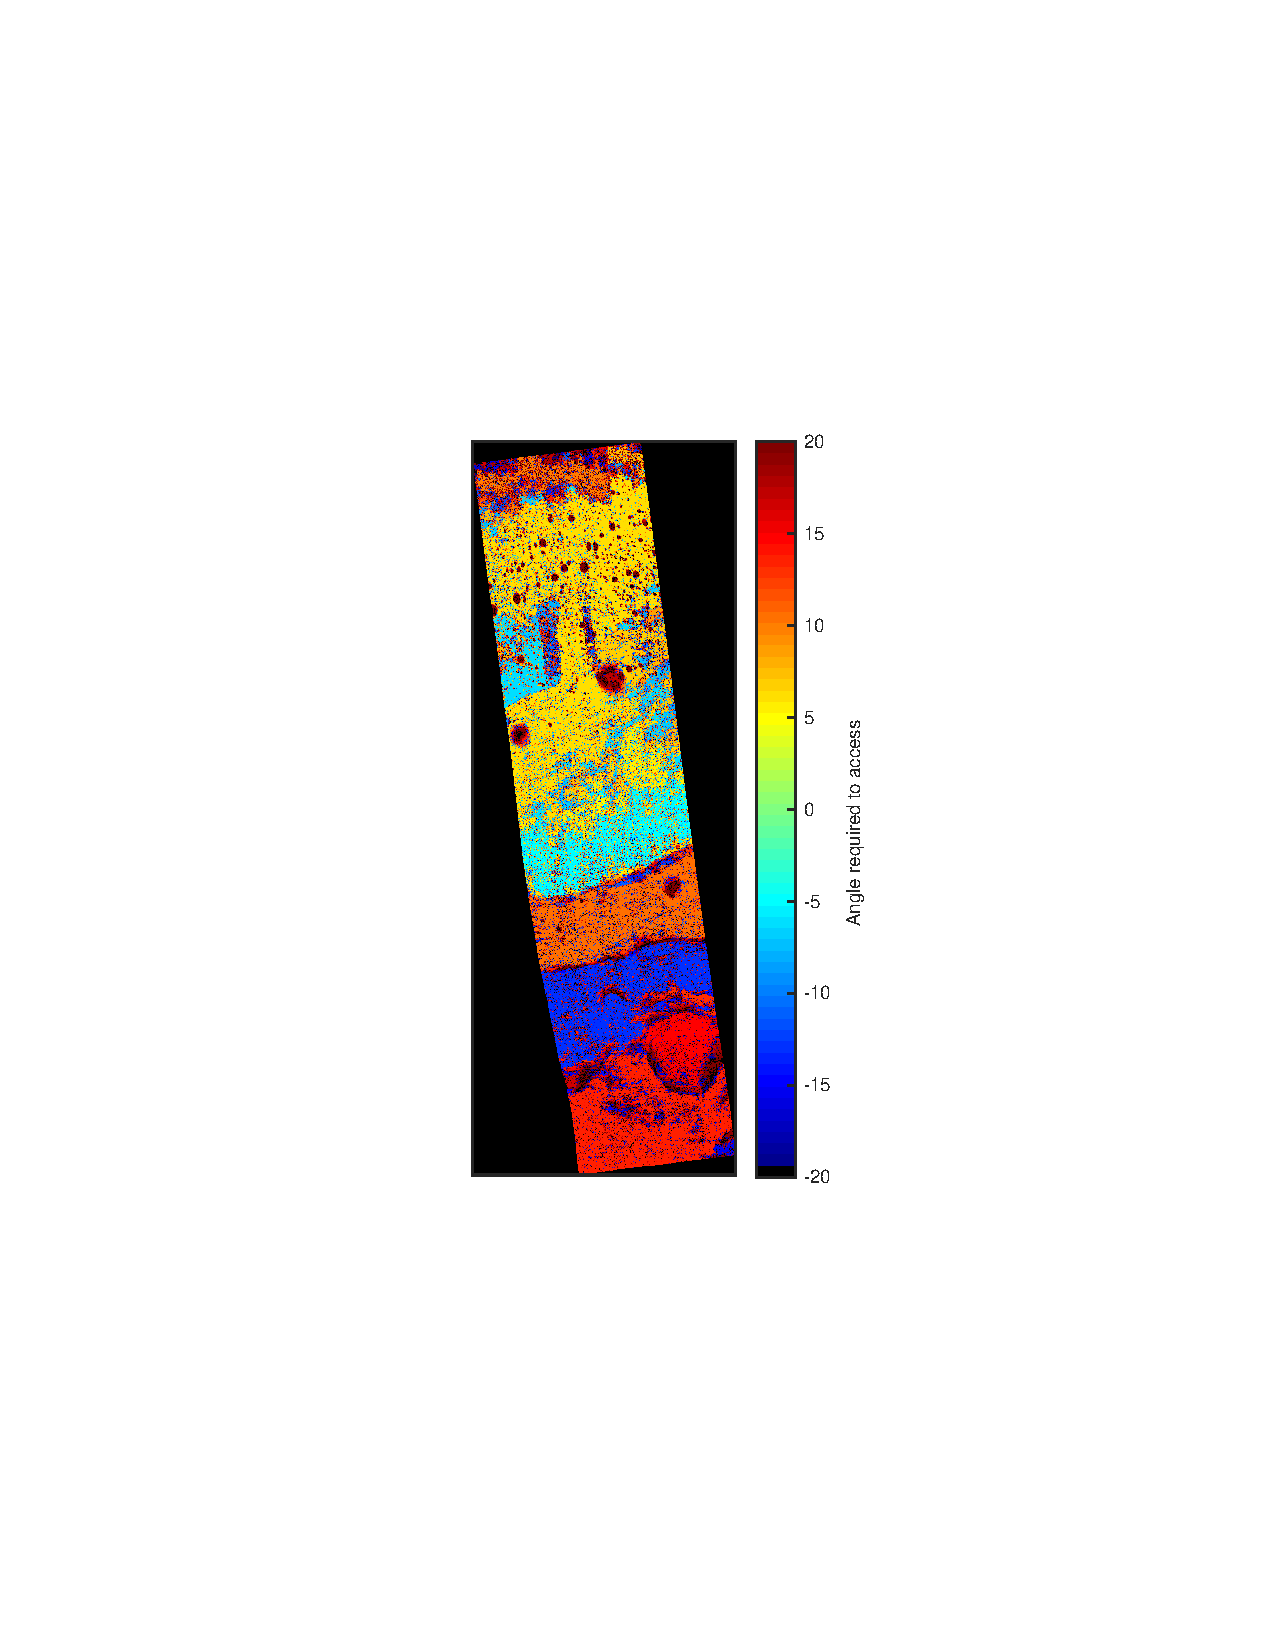
\includegraphics[height=0.4\paperheight]{figures/maps/ESP_011844_1855/DTEEC_011844_1855_002812_1855_A01-traversability_map.pdf}
    \caption{Traversability map}
    \label{fig:southwest_traversability}
  \end{subfigure}
  \caption{Southwest Arabia Terra Landing Site Traversability Map}
  \label{fig:southwest}
\end{figure}
\par Figure~\ref{fig:southwest_dtm} and Figure~\ref{fig:southwest_traversability} respectively show the colored DTM, and the output traversability map for the Southwest Arabia Terra landing site. This map shows some rather interesting features. As we can see, the dark blue and the dark red in lower third of the site seem to indicate that the area is completely inaccessible. There is a very clear dividing line between this third and the rest of the map. This line is reflected in the DTM, where there is a cliff face along it. It does appear that the algorithm highlights these features and handled the cliff face quite well. As for the upper half of the map, there also seems to be a less severe divide between the low basin in the middle, and the higher terrain. The rover needs to be able to climb at least 5\textdegree to access this area. Looking at the traversability histogram in Figure~\ref{fig:southwest_hist}, we see that there are still a lot of pixels beyond the $\pm$20\textdegree bound, and a large segment of the pixels are located between +10\textdegree and +20\textdegree, i.e. the orange band above the inaccessible area.
\begin{figure}[h!]
  \centering
  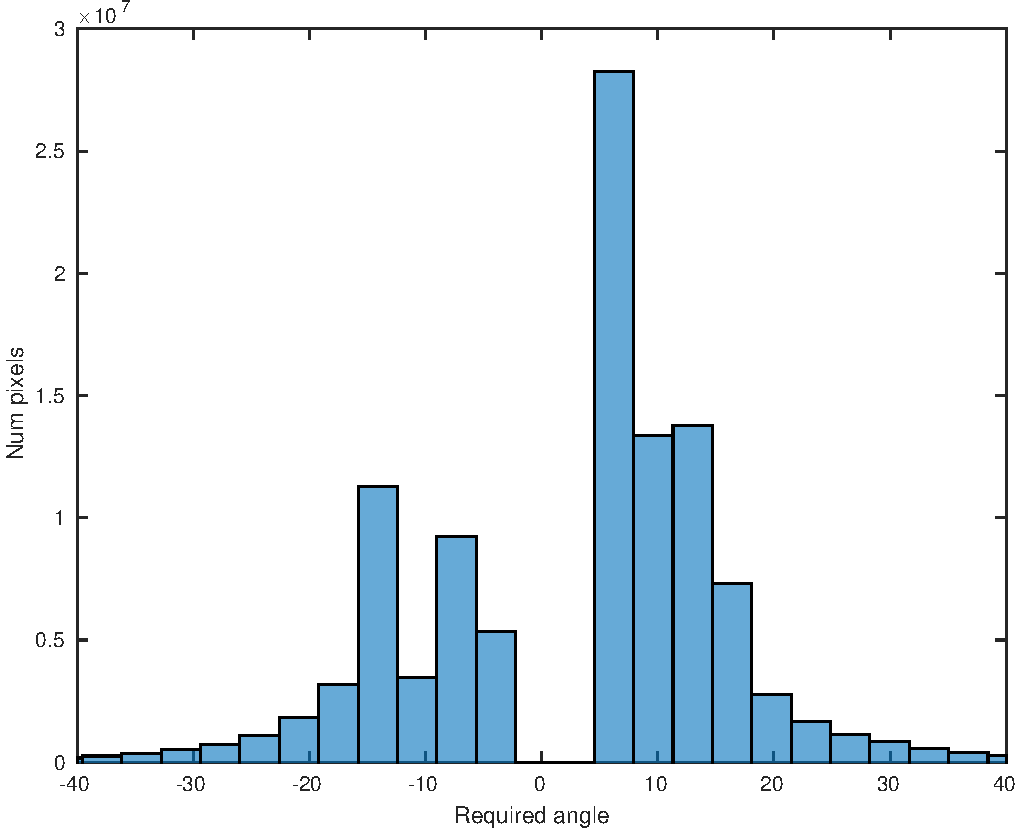
\includegraphics[width=0.6\textwidth]{figures/maps/ESP_011844_1855/DTEEC_011844_1855_002812_1855_A01-hist.pdf}
  \caption{Traversability Histogram for the Southwest Arabia Terra Landing Site}
  \label{fig:southwest_hist}
\end{figure}

\subsection{Mawrth Vallis\supcite{bib:ESP_015985_2040}}
\label{sub:mawrth_vallis}
\begin{figure}[h!]
  \centering
  \begin{subfigure}[t]{0.35\textwidth}
    \centering
    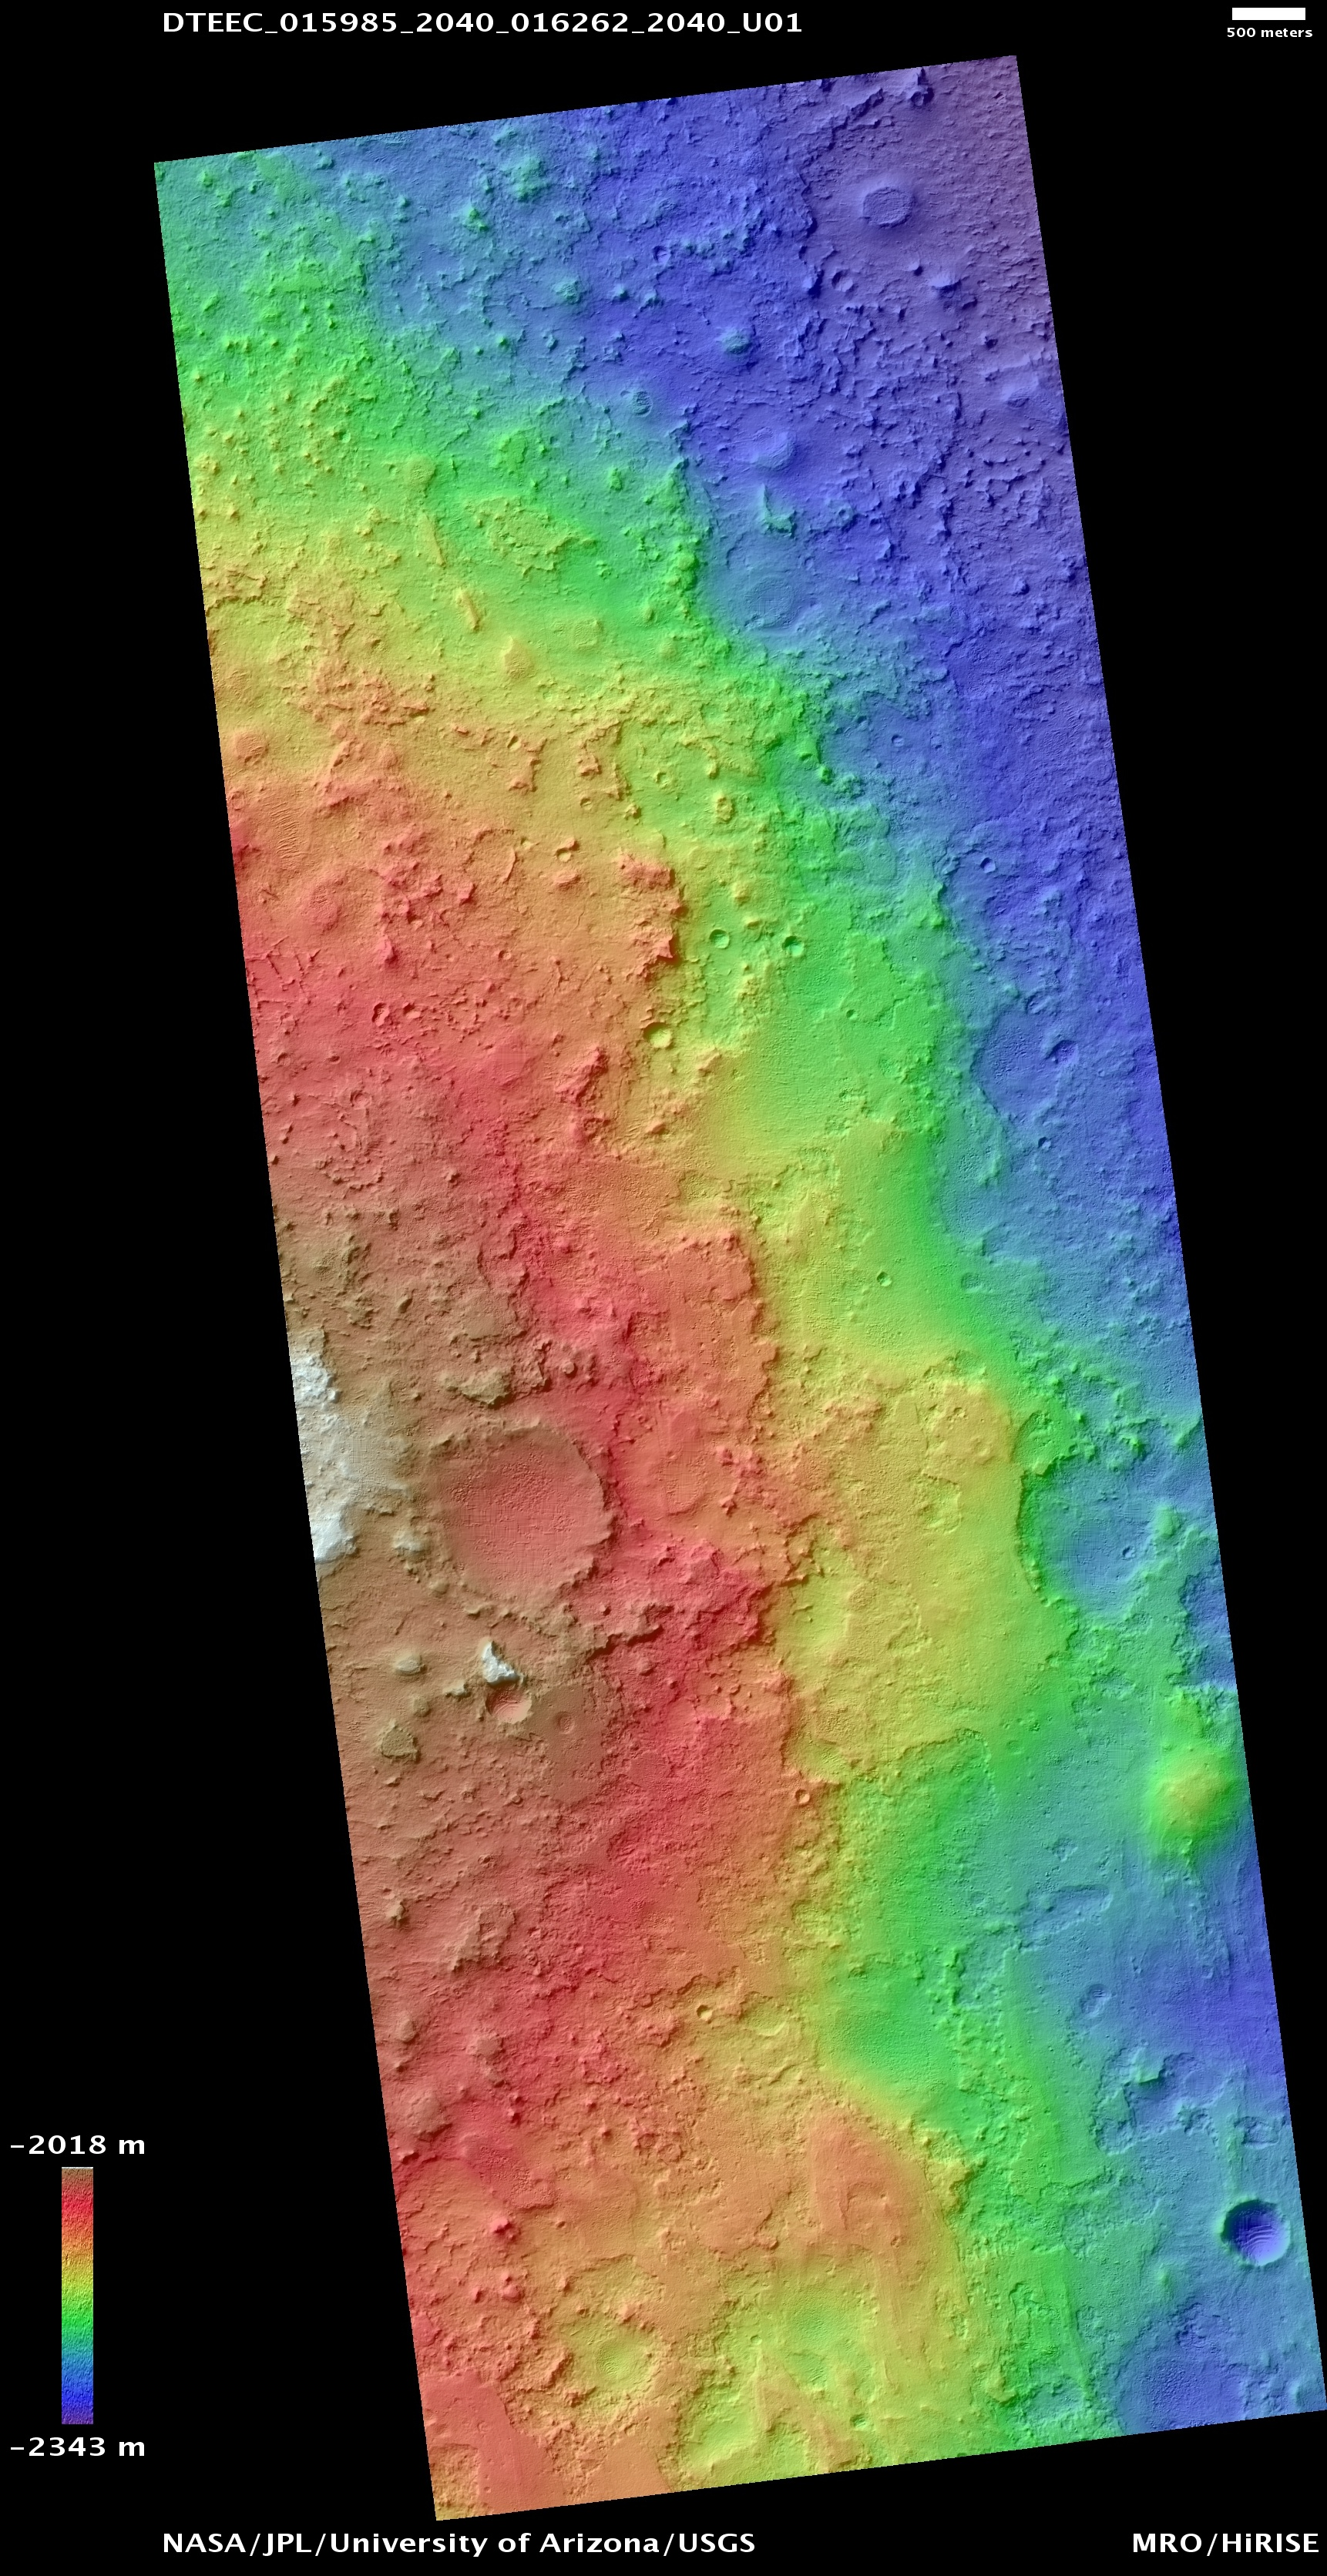
\includegraphics[height=0.4\paperheight]{figures/maps/ESP_015985_2040/DTEEC_015985_2040_016262_2040_U01.jpg}
    \caption{Color altimetry map}
    \label{fig:mawrth_dtm}
  \end{subfigure}
  ~
  \begin{subfigure}[t]{0.35\textwidth}
    \centering
    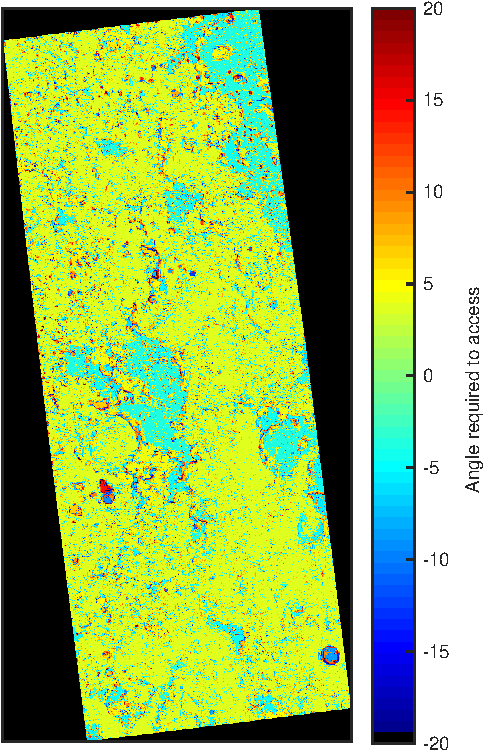
\includegraphics[height=0.4\paperheight]{figures/maps/ESP_015985_2040/DTEEC_015985_2040_016262_2040_U01-traversability_map.pdf}
    \caption{Traversability map}
    \label{fig:mawrth_traversability}
  \end{subfigure}
  \caption{Mawrth Vallis Landing Site Traversability Map}
  \label{fig:mawrth}
\end{figure}
\par This section of the Mawrth Vallis landing site was chosen because of its odd topography. The DTM in Figure~\ref{fig:mawrth_dtm} suggests that there are three distinct plateaus, and no guarantee that there exists a climbable path connecting them. In other words, if the rover were to land in the lowest plateau, it would never be able to gain access to the remaining ones, and vice versa. Fortunately, the traversability map in Figure~\ref{fig:mawrth_traversability} informs us that the entire section is in fact quite flat. Almost all of the traversability map is shaded in yellow or light blue, implying that those areas can be reached with a required angle of $\pm$5\textdegree. Looking at the histogram in Figure~\ref{fig:mawrth_hist}, 95\% of the landing site can be covered with a little less than $\pm$10\textdegree.
\begin{figure}[h!]
  \centering
  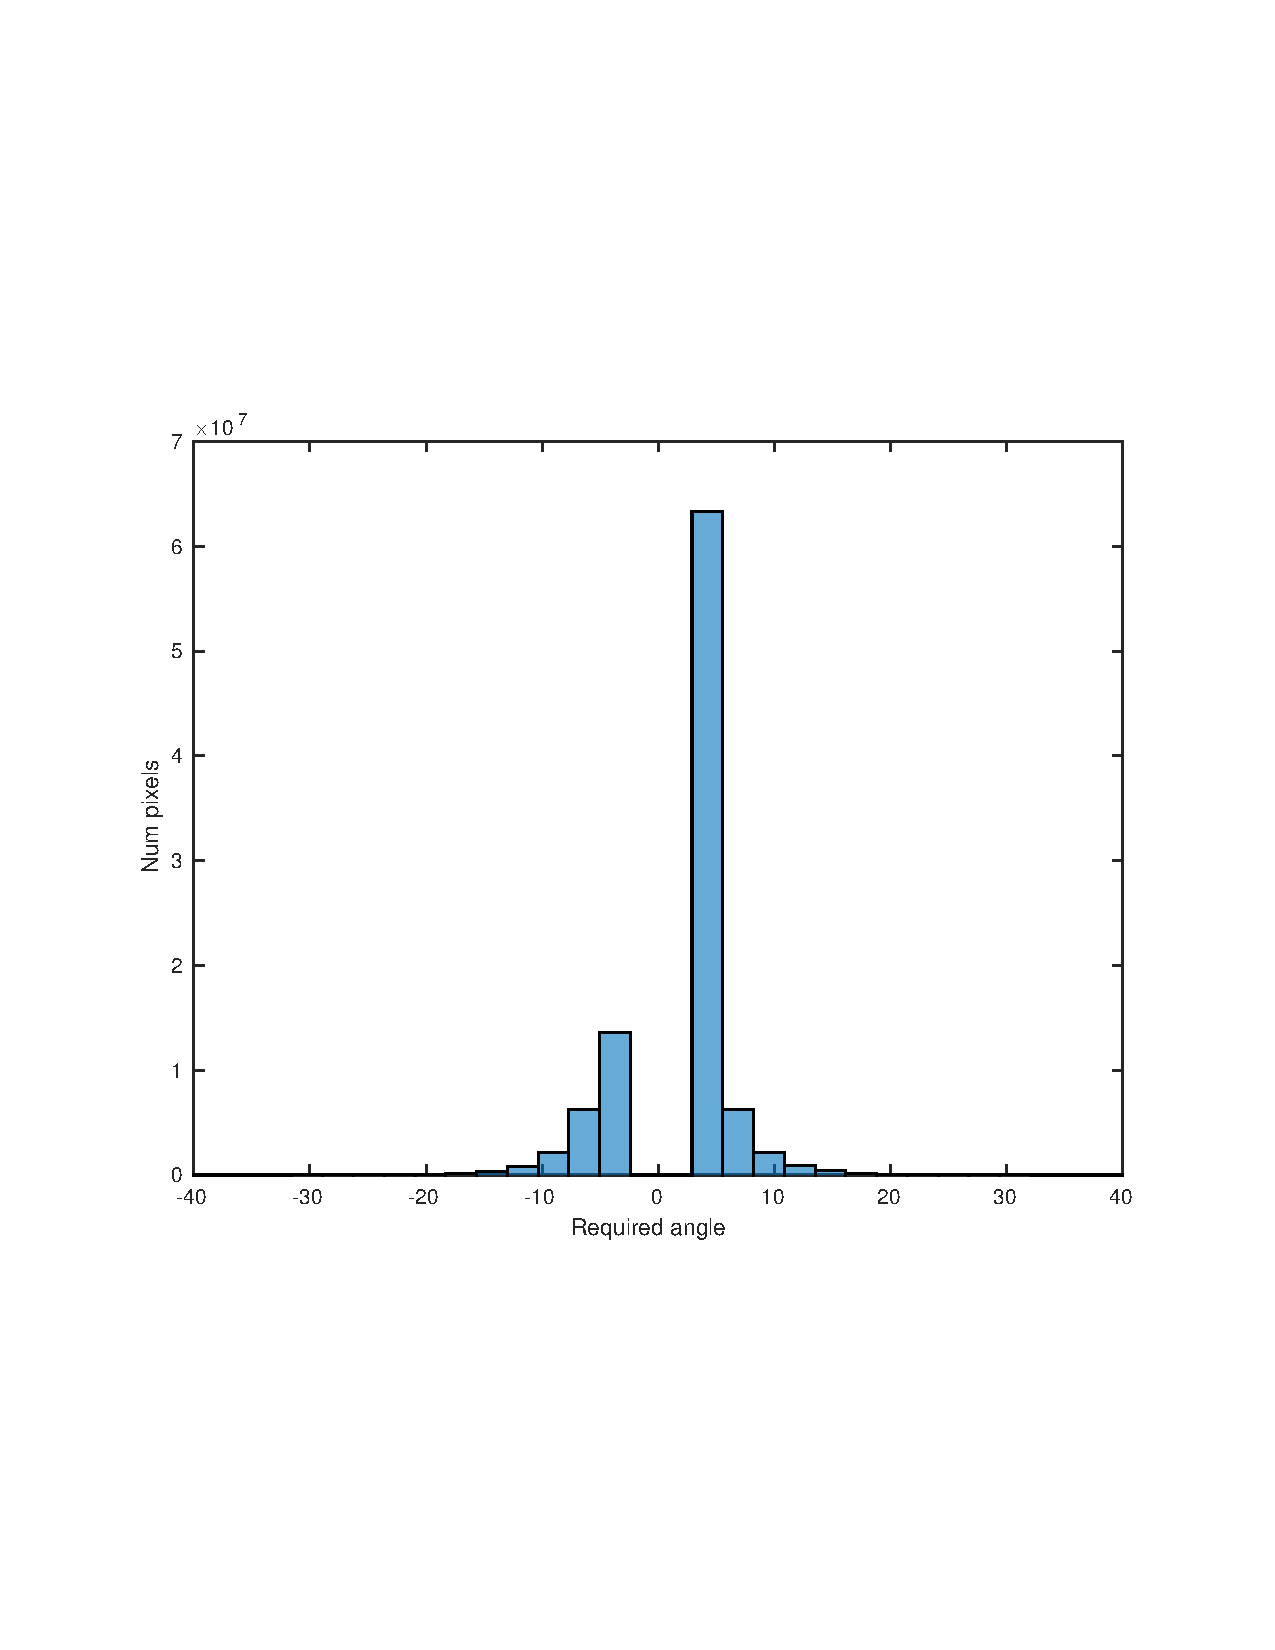
\includegraphics[width=0.6\textwidth]{figures/maps/ESP_015985_2040/DTEEC_015985_2040_016262_2040_U01-hist.pdf}
  \caption{Traversability Histogram for the Mawrth Vallis Landing Site}
  \label{fig:mawrth_hist}
\end{figure}

\subsection{Eberswalde, Gale and Holden Craters}
Please see figures \ref{fig:eberswalde}, \ref{fig:eberswalde_hist}, \ref{fig:gale}, \ref{fig:gale_hist}, \ref{fig:holden} and \ref{fig:holden_hist} in the Appendix for the DTMs, traversability maps and traversability histograms of the candidate landing sites in Eberswalde, Gale and Holden craters. Additionally, the code's \href{https://github.com/PapaCharlie/Rover-Climb-Angles/tree/master/figures/maps/}{\ttfamily\color{blue} \underline{source}} contains studies of more candidate sites.

\section{Weaknesses and Future Work}
\label{sec:weaknesses_and_future_work}
\par There are two major weaknesses in the current version of the algorithm.
\par As mentioned in the algorithm's definition, the starting position is always picked to be the middle of the DTM. Essentially, this means that the required angles shown in the map are actually the angles required to access those points had we started from the center. Fortunately, a lot of information can still be inferred from these maps, even with this slight subtlety. One of the ways to fix this problem would be to use as a starting point the actual target area for the site. A better method would be to pick multiple starting positions. In this case, the frontier of reachable points would start disconnected, then merge with its cousin as the algorithm progresses. This would give us better understanding of the terrain.
\par Another weakness in this algorithm is that it is a little naive. The difficulty in getting from point A to point B does not only lie in the angle of the slope between A and B. It also lies within the actual material the rover is going over. A slope of sand is harder to go over than a slope of gravel or rock. As such, one of the ways to improve this algorithm would be to keep track of a ``difficulty'' value of some sort, as opposed to only the angle. Suppose we had the albedo of the material at every point in addition to the height. With a mapping from albedo to terrain difficulty, it would be a matter of evaluating the ``difficulty'' rating of the slope between two points, for example by multiplying the terrain difficulty by the angle. In which case the values contained in the traversability maps would be more arbitrary, but be more informative.
\par As long as the data is provided, both of these modifications are implementable without too much overhead.

\section{Conclusion}
\label{sec:conclusion}
\par The goal of this proposal was to establish a pipeline takes DTMs at arbitrary precisions, and outputs the respective traversability maps in a reasonable. Given the more than successful results with the candidate landing sites, we can safely conclude that our goal has been achieved. The final product is a stable piece of software that outputs valuable information, though there is still room for improvement.
\par As for the landing sites presented in this paper, it would seem that Mawrth Vallis is a great candidate. It is flat and traversable, and given that it is one of the oldest valleys on Mars, is certainly a region of interest. On the other hand, landing sites such as the one near Southwest Arabia Terra appear to be much harder to traverse. Though it may contain valuable information, it is not necessarily a good choice if movement is hindered every step of the way. The traversability maps were created for the sole purpose of aiding the in the choice of landing site and rover design, and it appears that this pipeline would indeed be a useful tool in making those decision.

\clearpage
\begin{thebibliography}{30}
\bibitem{bib:rover2020}
  \url{http://mars.nasa.gov/mars2020/mission/rover/}
\bibitem{bib:curiosity}
  \url{http://mars.nasa.gov/msl/mission/rover/}
\bibitem{bib:hirise}
  \url{http://mars.nasa.gov/mro/mission/instruments/hirise/}
\bibitem{bib:abouthirise}
  \url{http://www.uahirise.org/dtm/about.php}
\bibitem{bib:nasa-review}
  \url{http://www.marsjournal.org/contents/2008/0002/files/som_mars_2008_0002.pdf}
\bibitem{bib:angle}
  \url{http://www.jpl.nasa.gov/news/news.php?feature=4596}
\bibitem{bib:hsrc}
  \url{http://pds-geosciences.wustl.edu/missions/mars_express/hrsc.htm}
\bibitem{bib:groundspeed}
  \url{http://www.space.com/22226-mars-rover-curiosity-time-lapse-video.html}
\bibitem{bib:ESP_011844_1855}
  \url{www.uahirise.org/dtm/dtm.php?ID=ESP_011844_1855}
\bibitem{bib:ESP_023957_1755}
  \url{www.uahirise.org/dtm/dtm.php?ID=ESP_023957_1755}
\bibitem{bib:ESP_019612_1535}
  \url{www.uahirise.org/dtm/dtm.php?ID=ESP_019612_1535}
\bibitem{bib:ESP_019757_1560}
  \url{www.uahirise.org/dtm/dtm.php?ID=ESP_019757_1560}
\bibitem{bib:ESP_015985_2040}
  \url{www.uahirise.org/dtm/dtm.php?ID=ESP_015985_2040}
\end{thebibliography}

\section{Appendix}
\label{sec:appendix}
\begin{figure}[h!]
  \centering
  \begin{subfigure}[t]{0.35\textwidth}
    \centering
    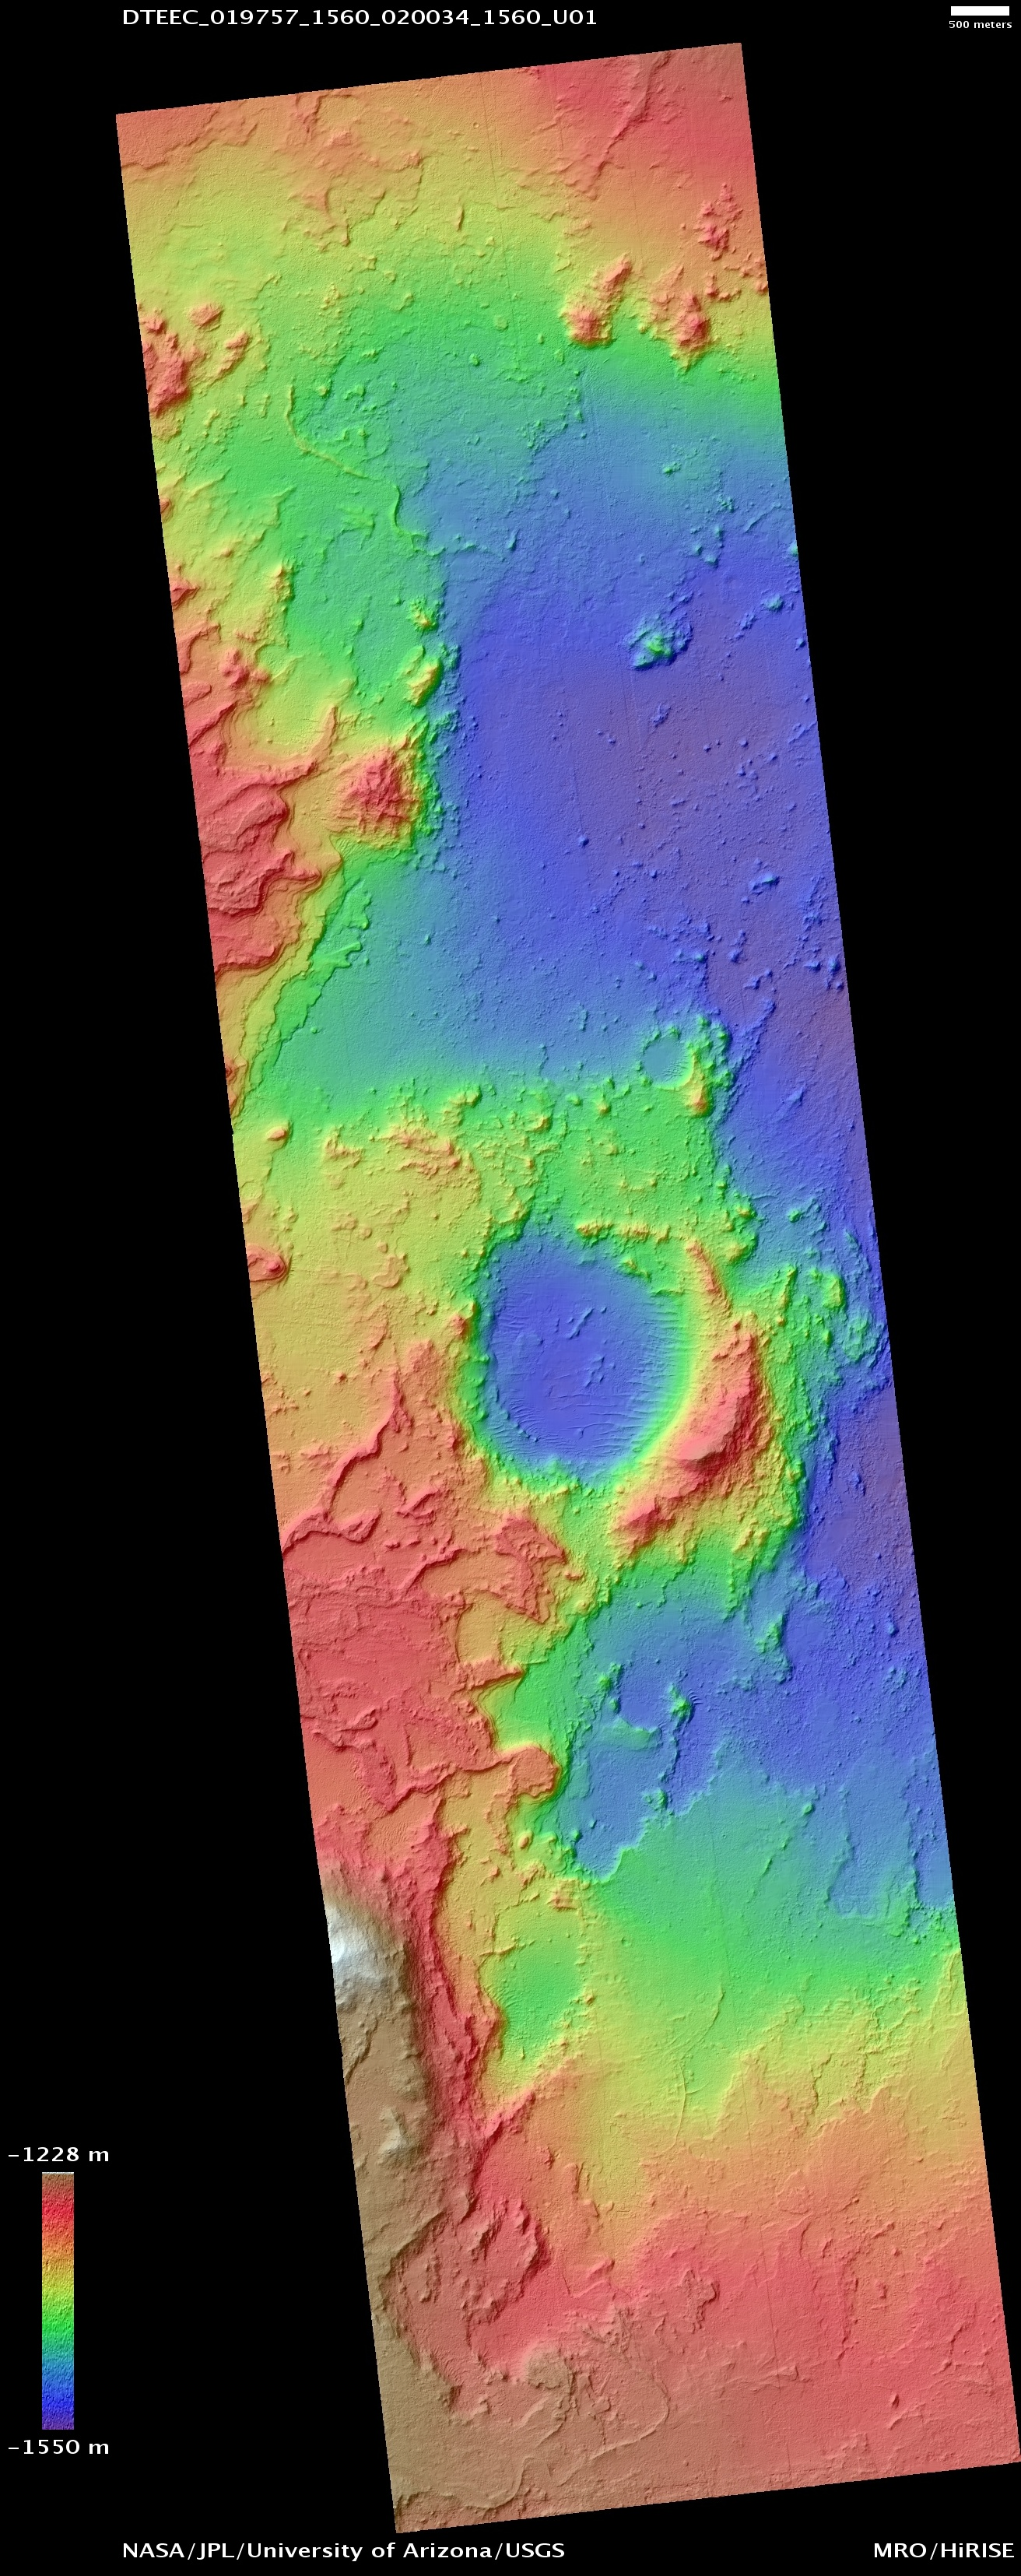
\includegraphics[height=0.4\paperheight]{figures/maps/ESP_019757_1560/DTEEC_019757_1560_020034_1560_U01.jpg}
    \caption{Color altimetry map}
    \label{fig:eberswalde_dtm}
  \end{subfigure}
  ~
  \begin{subfigure}[t]{0.35\textwidth}
    \centering
    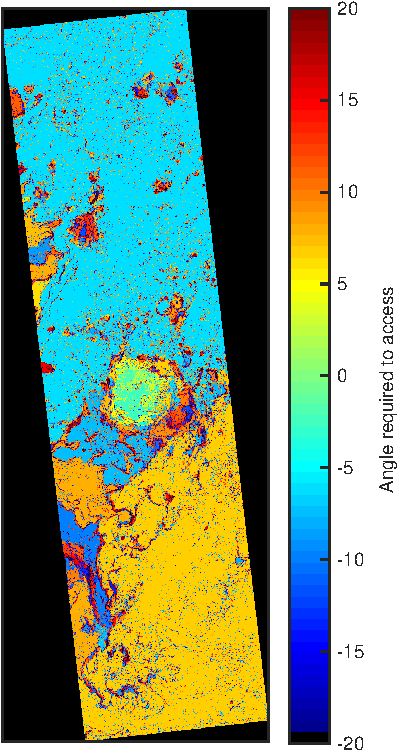
\includegraphics[height=0.4\paperheight]{figures/maps/ESP_019757_1560/DTEEC_019757_1560_020034_1560_U01-traversability_map.pdf}
    \caption{Traversability map}
    \label{fig:eberswalde_traversability}
  \end{subfigure}
  \caption{Mawrth Vallis Landing Site Traversability Map}
  \label{fig:eberswalde}
\end{figure}
\begin{figure}[h!]
  \centering
  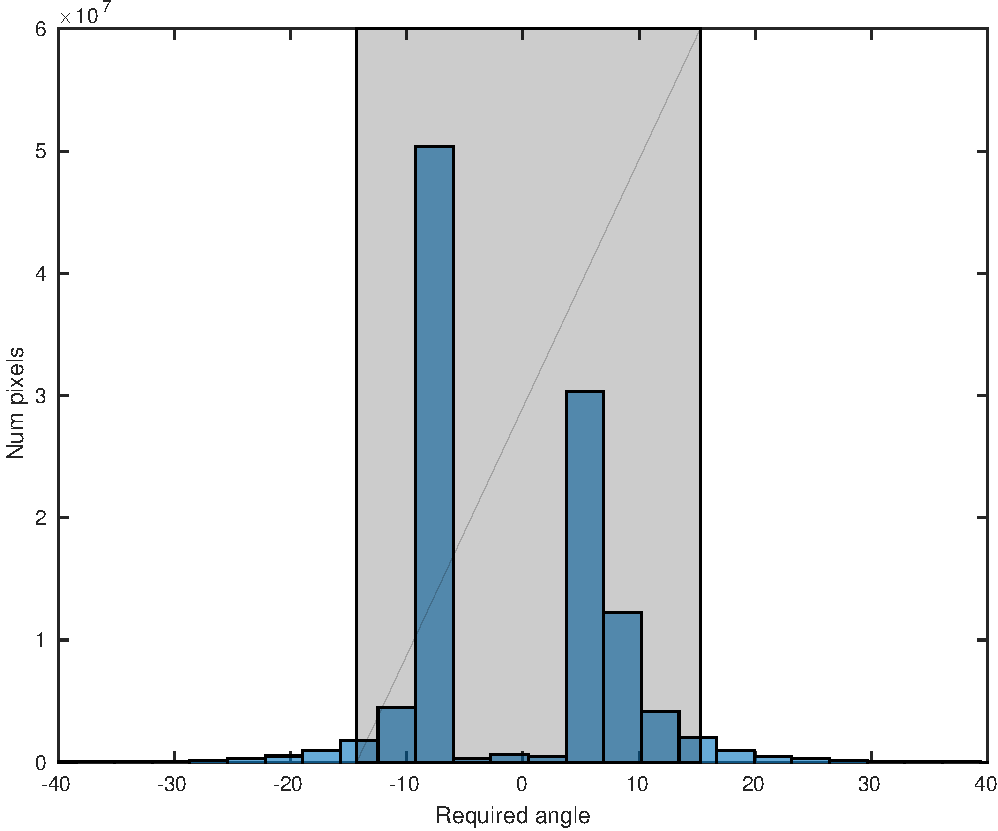
\includegraphics[width=0.6\textwidth]{figures/maps/ESP_019757_1560/DTEEC_019757_1560_020034_1560_U01-hist.pdf}
  \caption{Traversability Histogram for the Mawrth Vallis Landing Site}
  \label{fig:eberswalde_hist}
\end{figure}

\begin{figure}[h!]
  \centering
  \begin{subfigure}[t]{0.35\textwidth}
    \centering
    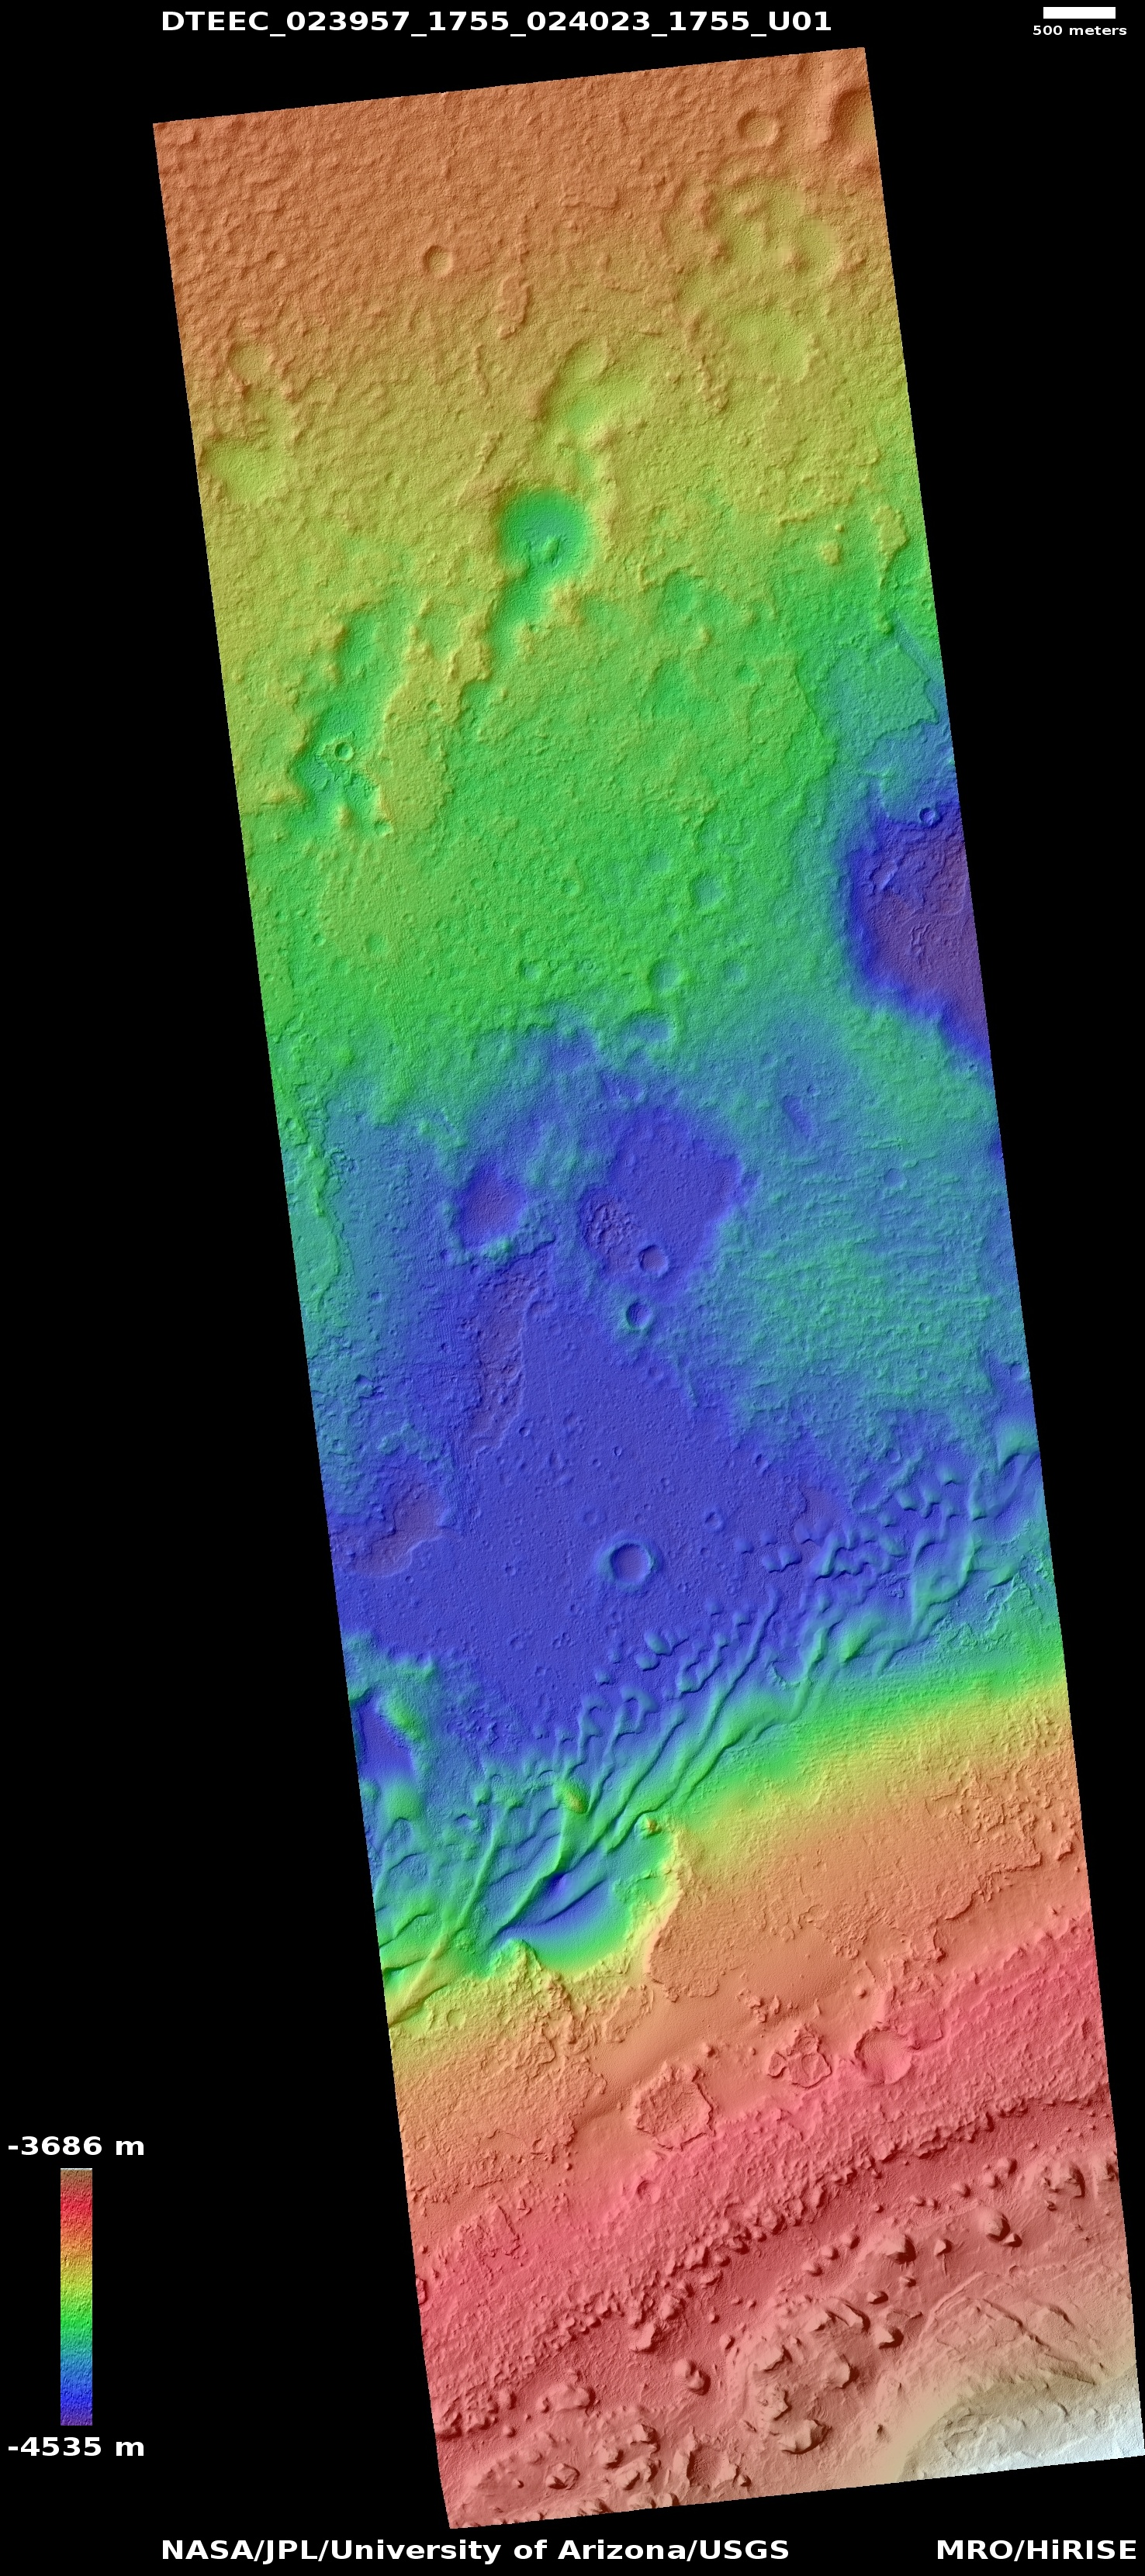
\includegraphics[height=0.4\paperheight]{figures/maps/ESP_023957_1755/DTEEC_023957_1755_024023_1755_U01.jpg}
    \caption{Color altimetry map}
    \label{fig:gale_dtm}
  \end{subfigure}
  ~
  \begin{subfigure}[t]{0.35\textwidth}
    \centering
    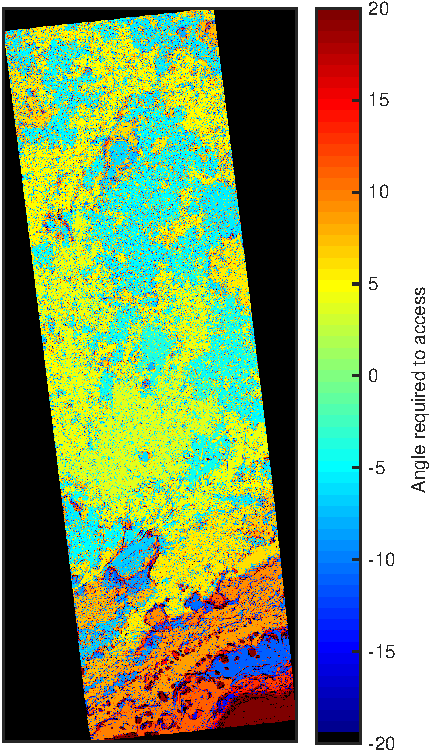
\includegraphics[height=0.4\paperheight]{figures/maps/ESP_023957_1755/DTEEC_023957_1755_024023_1755_U01-traversability_map.pdf}
    \caption{Traversability map}
    \label{fig:gale_traversability}
  \end{subfigure}
  \caption{Mawrth Vallis Landing Site Traversability Map}
  \label{fig:gale}
\end{figure}
\begin{figure}[h!]
  \centering
  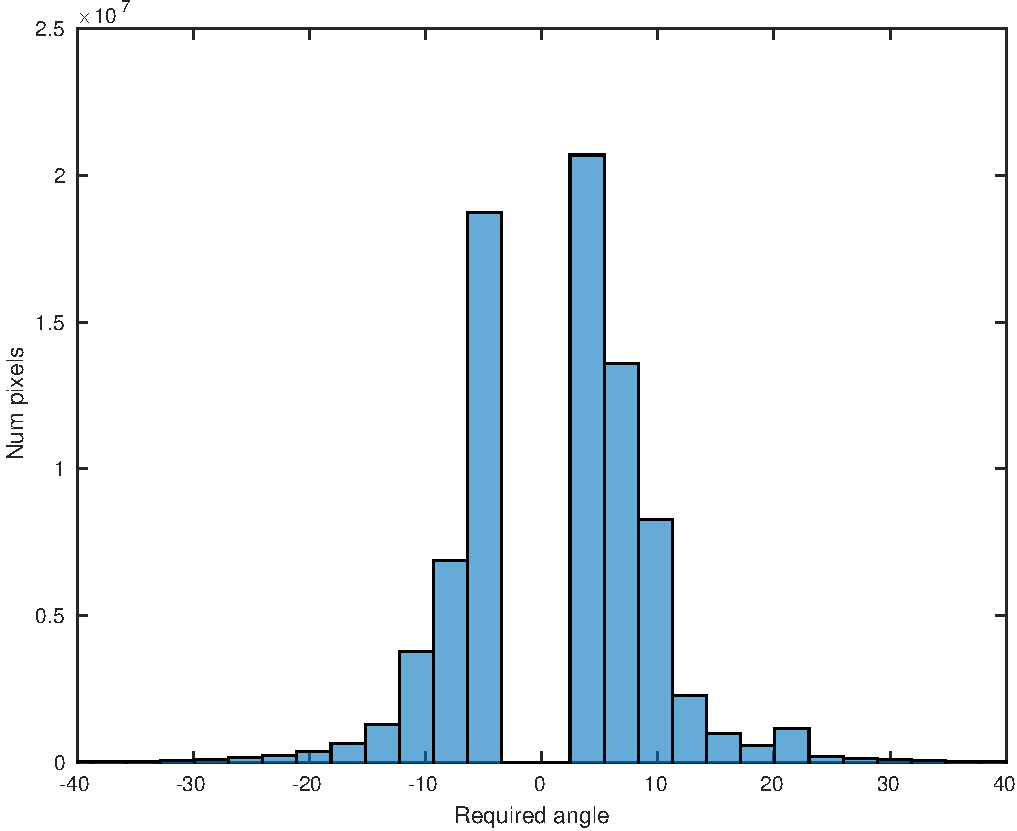
\includegraphics[width=0.6\textwidth]{figures/maps/ESP_023957_1755/DTEEC_023957_1755_024023_1755_U01-hist.pdf}
  \caption{Traversability Histogram for the Mawrth Vallis Landing Site}
  \label{fig:gale_hist}
\end{figure}

\begin{figure}[h!]
  \centering
  \begin{subfigure}[t]{0.35\textwidth}
    \centering
    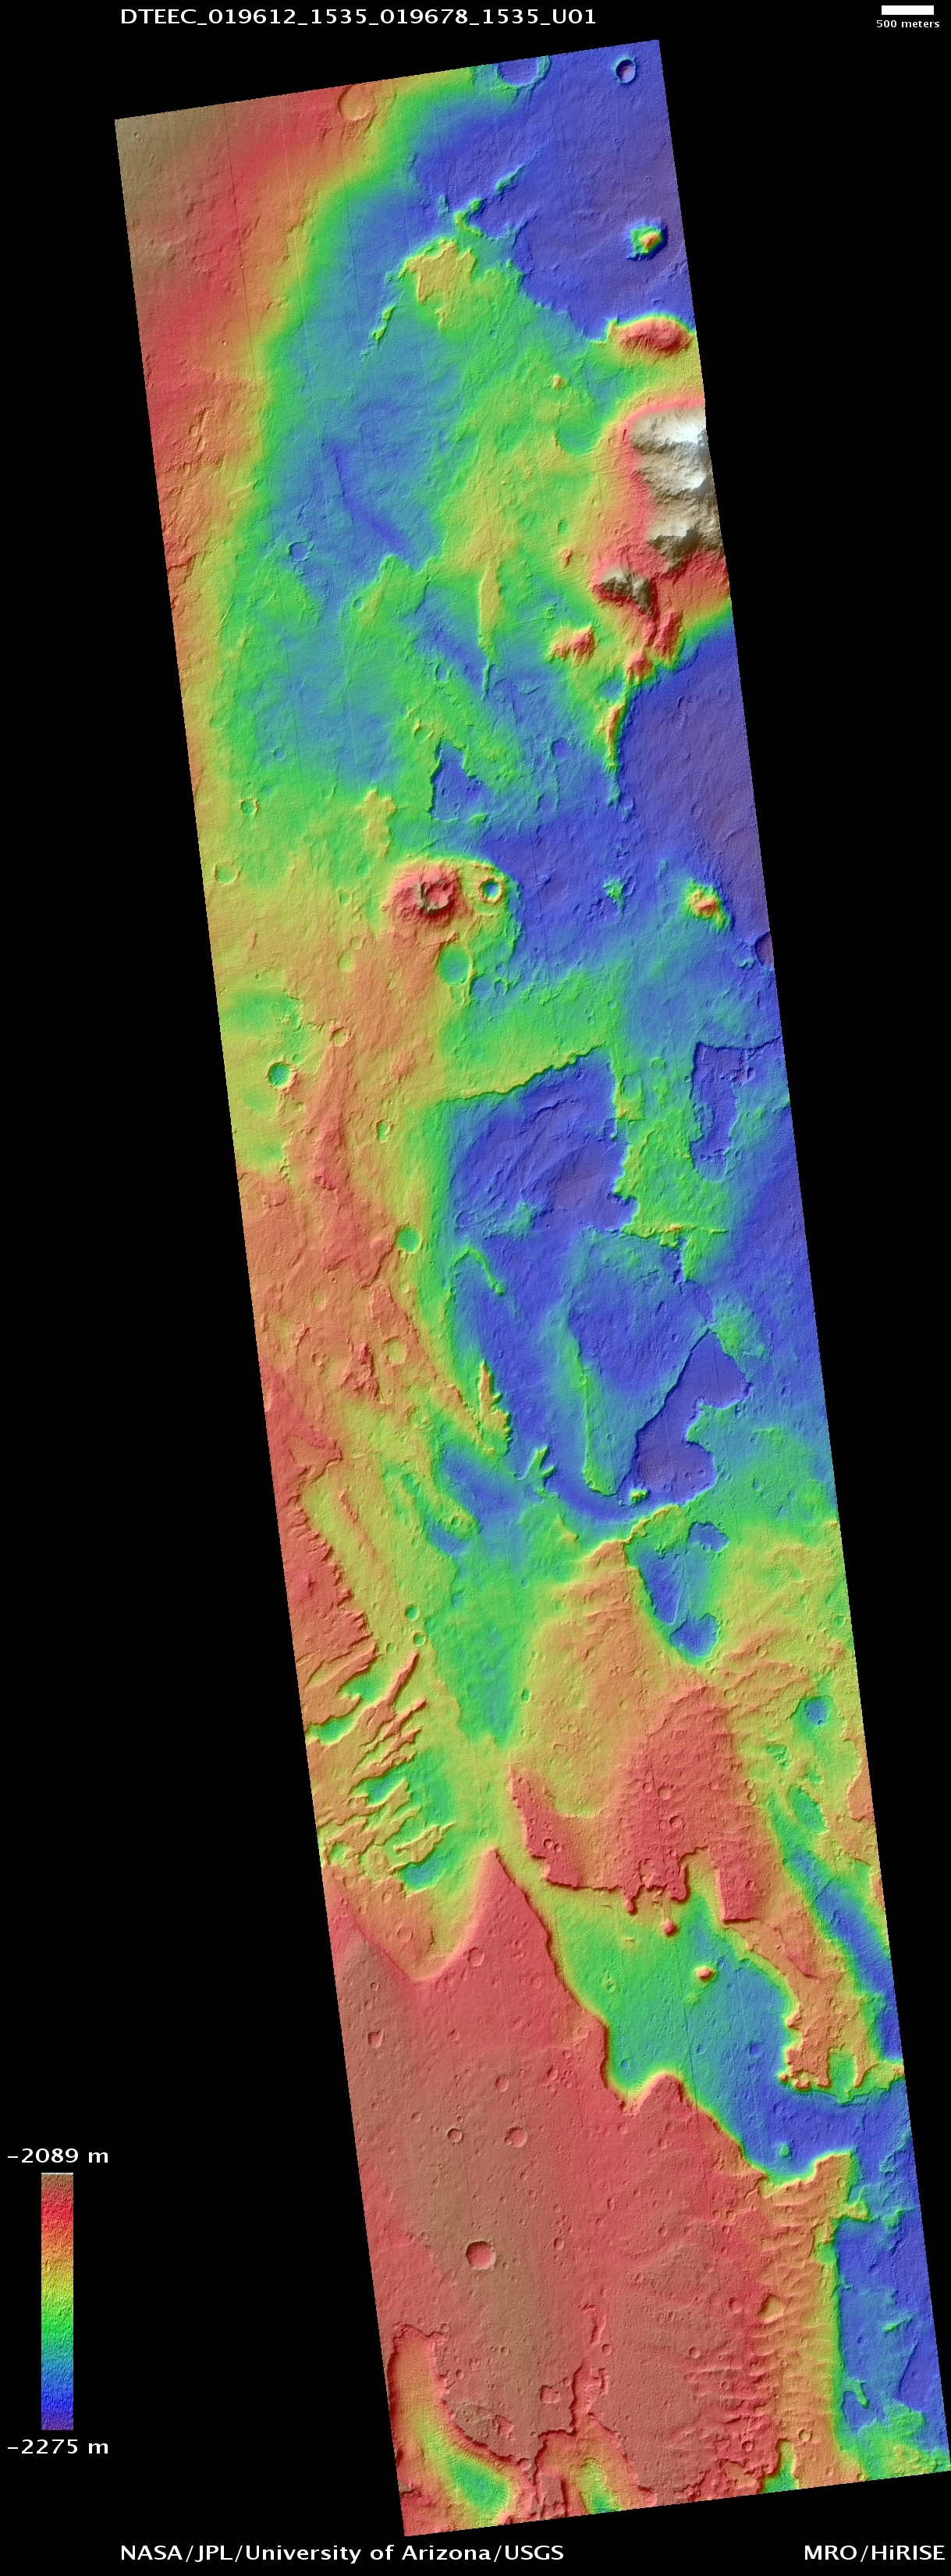
\includegraphics[height=0.4\paperheight]{figures/maps/ESP_019612_1535/DTEEC_019612_1535_019678_1535_U01.jpg}
    \caption{Color altimetry map}
    \label{fig:holden_dtm}
  \end{subfigure}
  ~
  \begin{subfigure}[t]{0.35\textwidth}
    \centering
    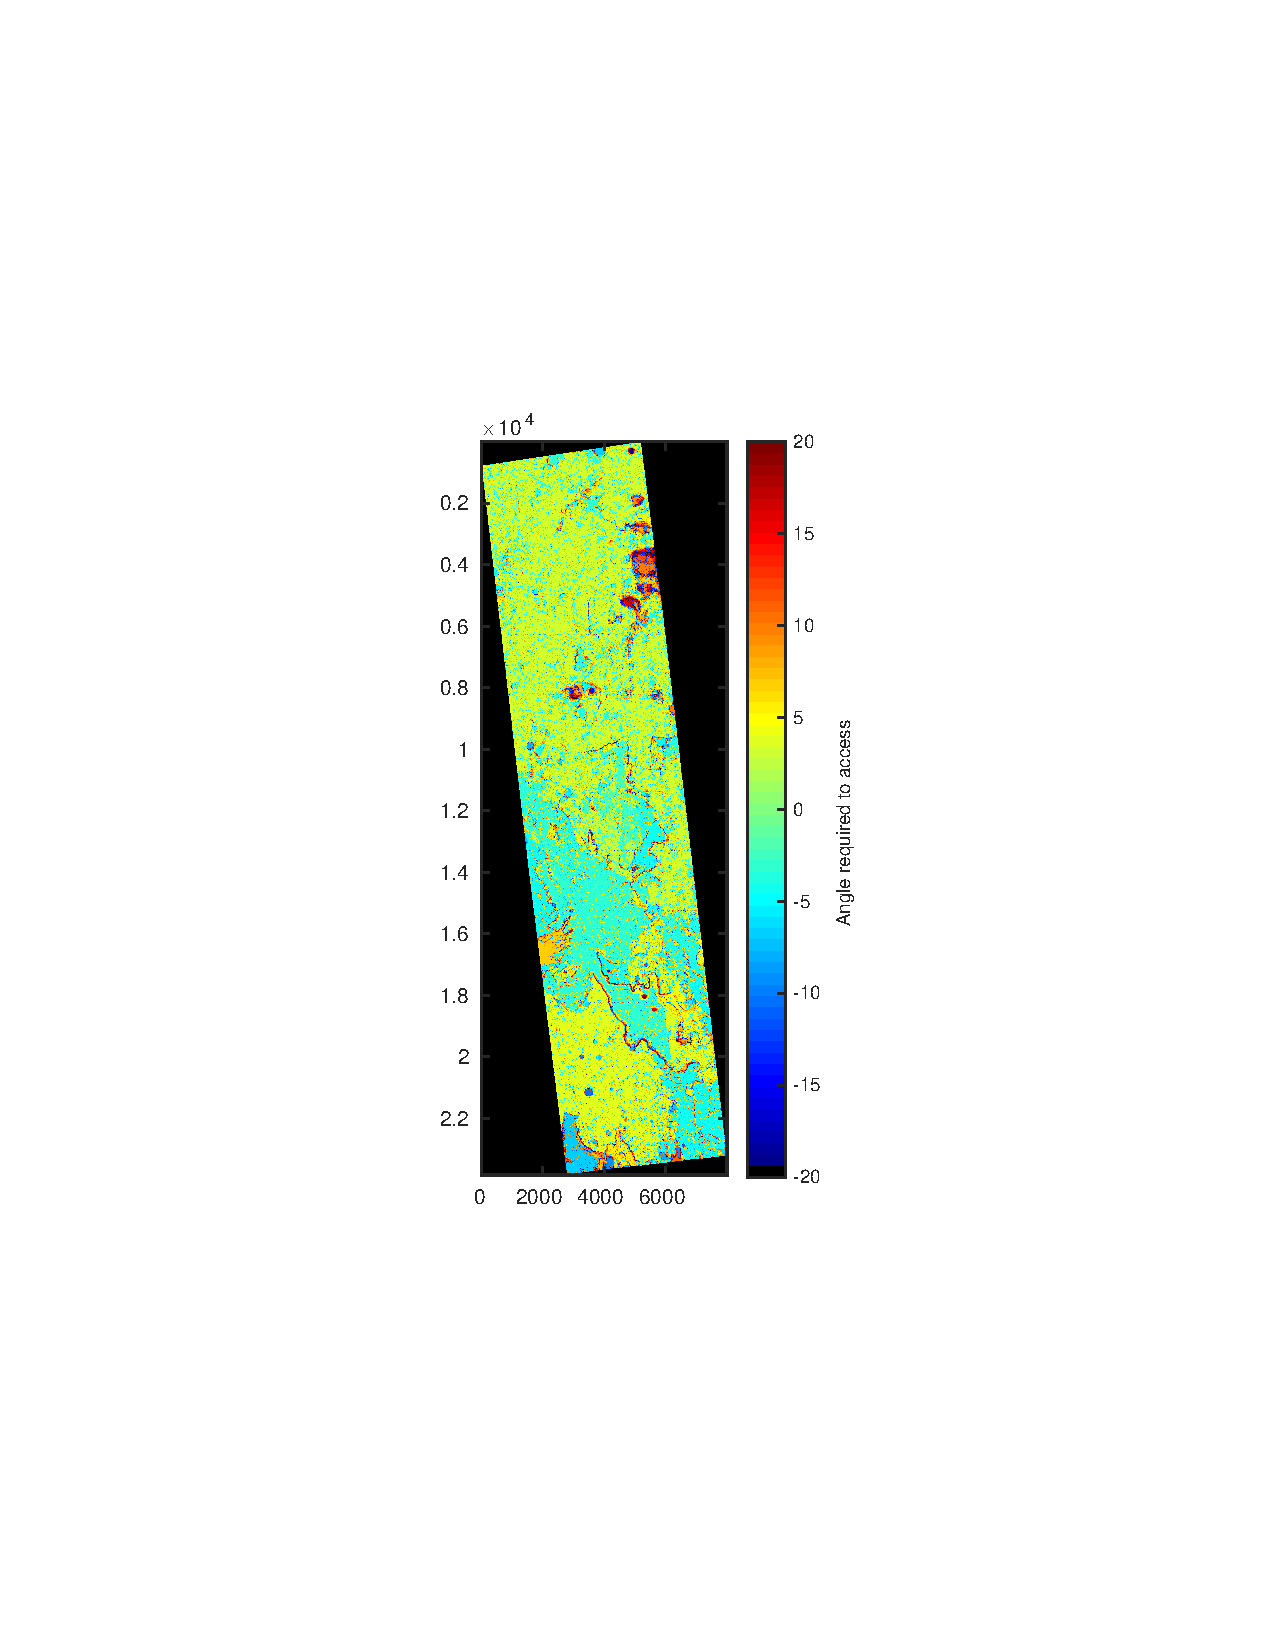
\includegraphics[height=0.4\paperheight]{figures/maps/ESP_019612_1535/DTEEC_019612_1535_019678_1535_U01-traversability_map.pdf}
    \caption{Traversability map}
    \label{fig:holden_traversability}
  \end{subfigure}
  \caption{Mawrth Vallis Landing Site Traversability Map}
  \label{fig:holden}
\end{figure}
\begin{figure}[h!]
  \centering
  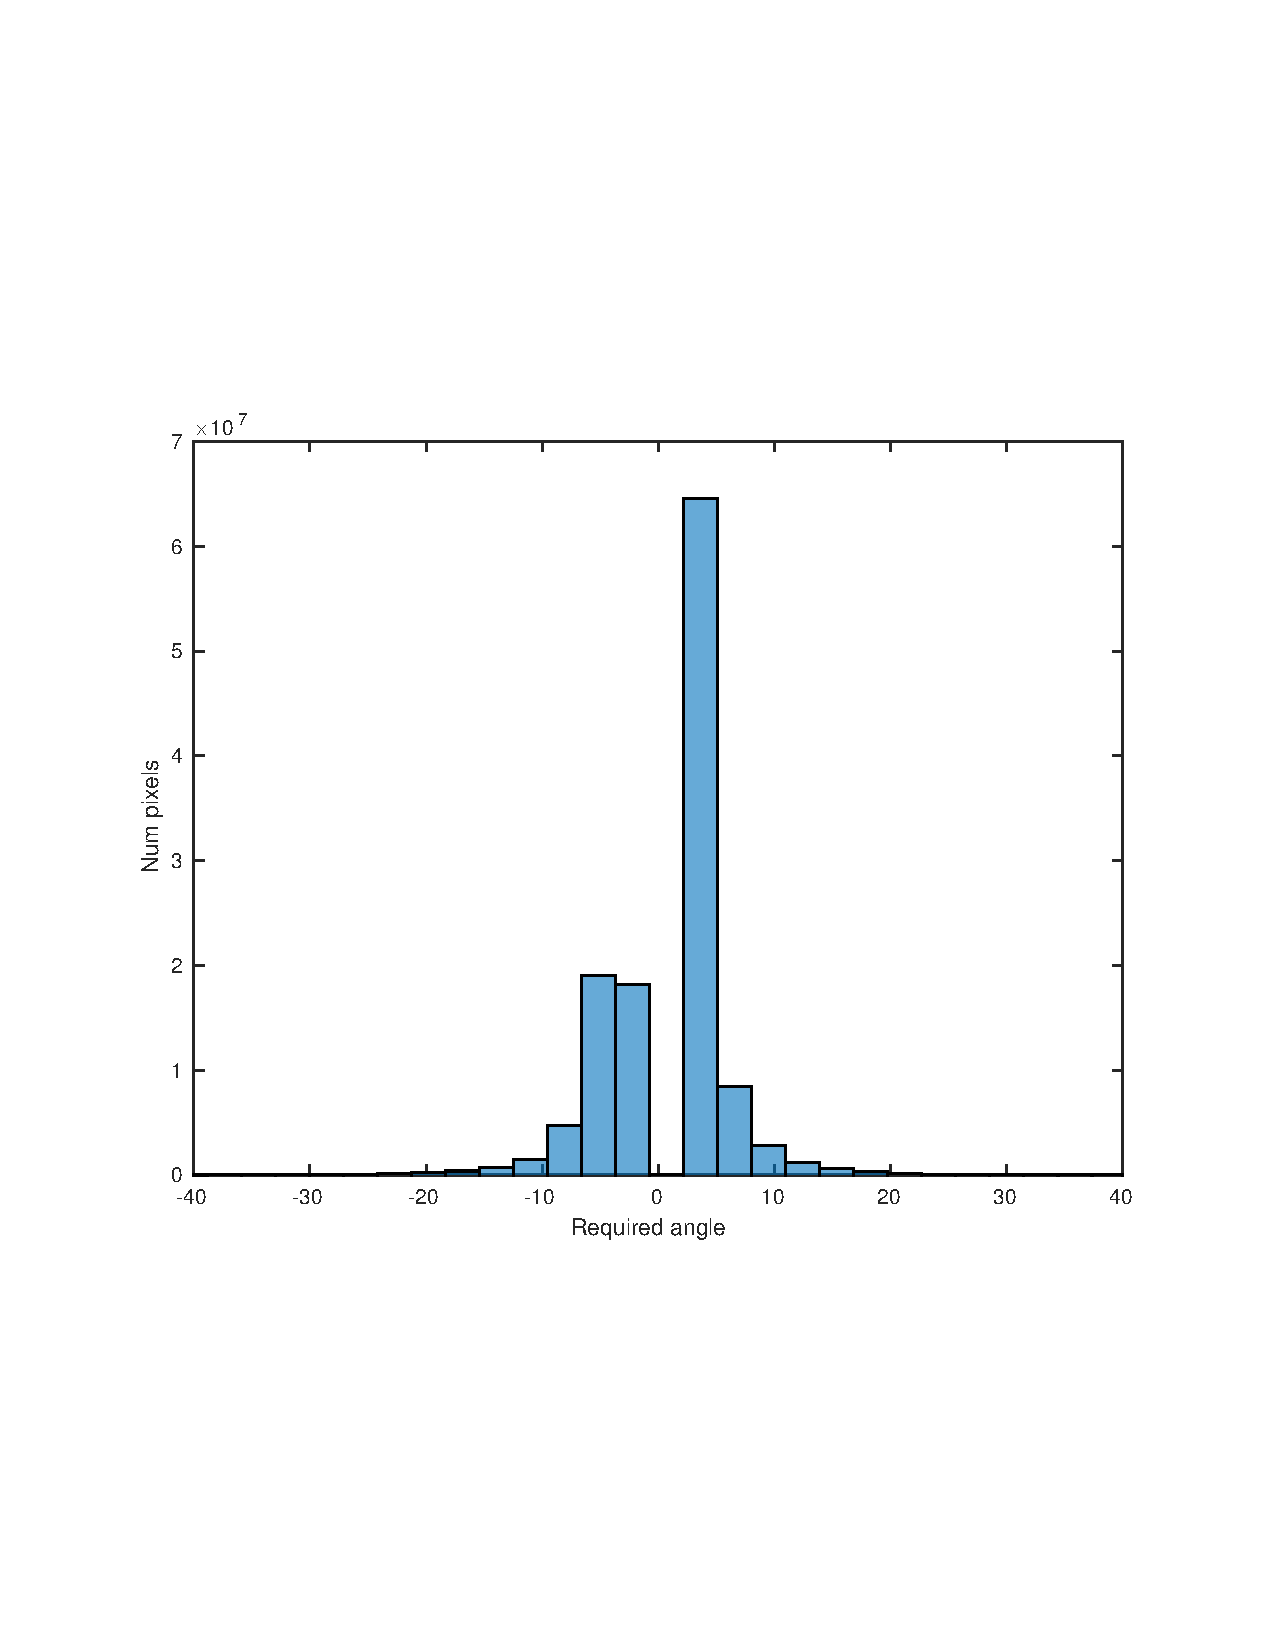
\includegraphics[width=0.6\textwidth]{figures/maps/ESP_019612_1535/DTEEC_019612_1535_019678_1535_U01-hist.pdf}
  \caption{Traversability Histogram for the Mawrth Vallis Landing Site}
  \label{fig:holden_hist}
\end{figure}

\end{document}
